% Huang's signed adjacency matrix of the cube Q_3: solid = +1, dashed red = -1. Every 4-cycle has an odd number of minus signs.
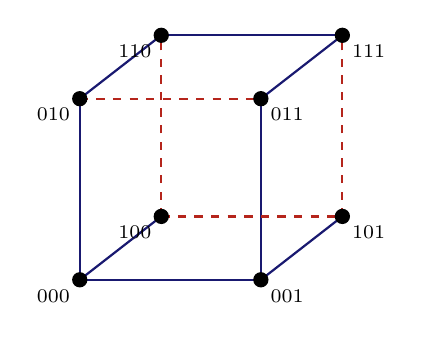
\begin{tikzpicture}[scale=1.15]
\draw[MidnightBlue,thick] (0.00,0.00) -- (2.00,0.00);
\draw[MidnightBlue,thick] (0.00,0.00) -- (0.00,2.00);
\draw[MidnightBlue,thick] (0.00,0.00) -- (0.90,0.70);
\draw[MidnightBlue,thick] (2.00,0.00) -- (2.00,2.00);
\draw[MidnightBlue,thick] (2.00,0.00) -- (2.90,0.70);
\draw[BrickRed,thick,dashed] (0.00,2.00) -- (2.00,2.00);
\draw[MidnightBlue,thick] (0.00,2.00) -- (0.90,2.70);
\draw[MidnightBlue,thick] (2.00,2.00) -- (2.90,2.70);
\draw[BrickRed,thick,dashed] (0.90,0.70) -- (2.90,0.70);
\draw[BrickRed,thick,dashed] (0.90,0.70) -- (0.90,2.70);
\draw[BrickRed,thick,dashed] (2.90,0.70) -- (2.90,2.70);
\draw[MidnightBlue,thick] (0.90,2.70) -- (2.90,2.70);
\fill[black] (0.000,0.000) circle (2.40pt);
\node[font=\scriptsize,anchor=north east] at (0.00,0.00) {$000$};
\fill[black] (2.000,0.000) circle (2.40pt);
\node[font=\scriptsize,anchor=north west] at (2.00,0.00) {$001$};
\fill[black] (0.000,2.000) circle (2.40pt);
\node[font=\scriptsize,anchor=north east] at (0.00,2.00) {$010$};
\fill[black] (2.000,2.000) circle (2.40pt);
\node[font=\scriptsize,anchor=north west] at (2.00,2.00) {$011$};
\fill[black] (0.900,0.700) circle (2.40pt);
\node[font=\scriptsize,anchor=north east] at (0.90,0.70) {$100$};
\fill[black] (2.900,0.700) circle (2.40pt);
\node[font=\scriptsize,anchor=north west] at (2.90,0.70) {$101$};
\fill[black] (0.900,2.700) circle (2.40pt);
\node[font=\scriptsize,anchor=north east] at (0.90,2.70) {$110$};
\fill[black] (2.900,2.700) circle (2.40pt);
\node[font=\scriptsize,anchor=north west] at (2.90,2.70) {$111$};
\end{tikzpicture}
